% FOC full-loop cascade block diagram.
% Compile: pdflatex foc-full-loop.tex && pdf2svg foc-full-loop.pdf foc-full-loop.svg
\documentclass[tikz, margin=4mm]{standalone}
\usetikzlibrary{arrows.meta, positioning, calc}

\tikzset{
  block/.style  = {draw, rectangle, rounded corners=2pt, align=center,
                   fill=blue!8, font=\small,
                   minimum height=1.1cm, minimum width=2.4cm},
  sum/.style    = {draw, circle, fill=blue!8, minimum size=7mm, inner sep=0pt},
  arr/.style    = {-{Latex[length=4pt, width=5pt]}, thick},
  lbl/.style    = {font=\footnotesize},
  node distance = 1.0cm and 1.8cm
}

\begin{document}
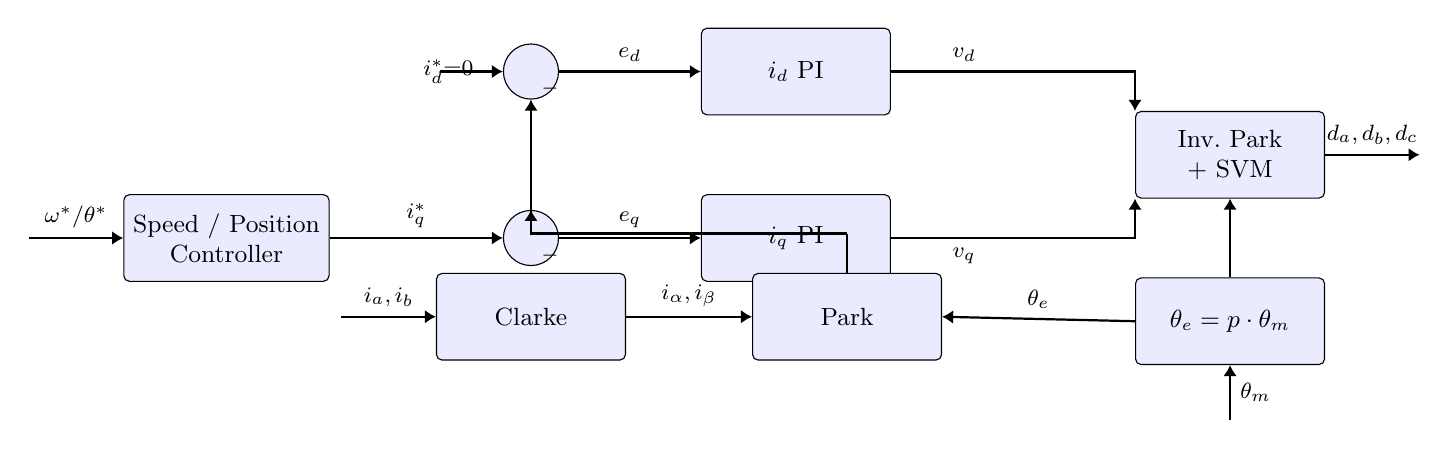
\begin{tikzpicture}

  % ── Current-loop core ─────────────────────────────────────────────────────
  \node[sum]                           (Sd)     {};
  \node[sum, below=1.4cm of Sd]        (Sq)     {};
  \node[block, right=1.8cm of Sd]      (Pd)     {$i_d$ PI};
  \node[block, right=1.8cm of Sq]      (Pq)     {$i_q$ PI};
  % mid-point between the two PIs
  \coordinate (midP) at ($(Pd.east)!0.5!(Pq.east)+(1.1,0)$);
  \node[block, right=2.0cm of midP, anchor=west] (InvP)
        {Inv.\ Park\\ $+$ SVM};

  % ── Outer speed / position loop ───────────────────────────────────────────
  \node[block, left=2.2cm of Sq]       (Outer)  {Speed / Position\\ Controller};

  % ── Sensing (bottom row) ──────────────────────────────────────────────────
  \node[block, below=2.2cm of Sd]      (Clarke) {Clarke};
  \node[block, right=1.6cm of Clarke]  (Park)   {Park};
  \node[block, below=1.0cm of InvP]    (Angle)  {$\theta_e = p \cdot \theta_m$};

  % ── I/O coordinates ───────────────────────────────────────────────────────
  \node[lbl, left=0.25cm of Sd, anchor=east]   {$i_d^* {=} 0$};
  \coordinate (IdRef)  at ($(Sd.west)+(-0.8,0)$);
  \coordinate (RefIn)  at ($(Outer.west)+(-1.2,0)$);
  \coordinate (AdcIn)  at ($(Clarke.west)+(-1.2,0)$);
  \coordinate (EncIn)  at ($(Angle.south)+(0,-0.7)$);
  \coordinate (PwmOut) at ($(InvP.east)+(1.2,0)$);

  % ── Connections ───────────────────────────────────────────────────────────

  % outer loop reference
  \draw[arr] (RefIn)  -- node[lbl,above]{$\omega^*/\theta^*$} (Outer);
  \draw[arr] (Outer)  -- node[lbl,above]{$i_q^*$}             (Sq);
  % id reference
  \draw[arr] (IdRef)  -- (Sd);

  % current PIDs → Inv. Park
  \draw[arr] (Sd) -- node[lbl,above]{$e_d$} (Pd);
  \draw[arr] (Sq) -- node[lbl,above]{$e_q$} (Pq);
  \draw[arr] (Pd.east) -| node[lbl,above,pos=0.15]{$v_d$} (InvP.north west);
  \draw[arr] (Pq.east) -| node[lbl,below,pos=0.15]{$v_q$} (InvP.south west);
  \draw[arr] (InvP.east) -- node[lbl,above]{$d_a,d_b,d_c$} (PwmOut);

  % ADC → Clarke → Park
  \draw[arr] (AdcIn)  -- node[lbl,above]{$i_a,i_b$}        (Clarke);
  \draw[arr] (Clarke) -- node[lbl,above]{$i_\alpha,i_\beta$} (Park);

  % Park feedback to summing junctions
  \coordinate (Pfb) at ($(Park.north)+(0,0.5)$);
  \draw (Park.north) -- (Pfb);
  \draw[arr] (Pfb) -| (Sd) node[below right, font=\scriptsize]{$-$};
  \draw[arr] (Pfb -| Sq) -- (Sq) node[below right, font=\scriptsize]{$-$};

  % Encoder → angle → Park and Inv. Park
  \draw[arr] (EncIn)  -- node[lbl,right]{$\theta_m$}  (Angle);
  \draw[arr] (Angle.west) -- node[lbl,above]{$\theta_e$} (Park.east);
  % θe branch to Inv. Park
  \coordinate (AtoInvP) at ($(Angle.north)+(0,0.35)$);
  \draw (Angle.north) -- (AtoInvP);
  \coordinate (AtoInvP_h) at (AtoInvP -| InvP.south);
  \draw[arr] (AtoInvP) -- (AtoInvP_h) -- (InvP.south);

\end{tikzpicture}
\end{document}
